\documentclass[11pt]{article}
%Gummi|065|=)
\title{Homework \#2: Discussion on kNN and Decision Trees\\ for Classifying CNN News Articles}
\author{Doug McGeehan\\
		CS 6001: Applied Spatial and \\ Temporal Data Analysis\\
		Spring 2017}

\usepackage[margin=1in]{geometry}
\usepackage{verbatim}
\usepackage{framed}
\usepackage{amsmath}
\usepackage{amssymb}
\usepackage{graphicx}
\usepackage{caption}
\usepackage{subcaption}

\begin{document}

\maketitle

\section{Experimental Setup}

100 articles from the CNN website were transformed into term frequency and tf-idf matrices for this report's analyses.
These articles were selected randomly in such a way as to have an equal portion of articles in each category: since there are seven categories present in the CNN article dataset, each category in the subset of 100 articles consists of 14 to 15 articles.
The results from each experiment were averaged through 5-fold cross validation,
 whereby the dataset was partitioned into five equal-sized subsets, four used for classifier training and one used for classifier testing.
This was repeated five times for all combinations of testing and training partition assignment.
The \texttt{scikit-learn} Python library was used to calculate the precision, recall, and f-scores of each classification task.

\section{Performance of Decision Trees}

The \texttt{DecisionTreeClassifier} of the \texttt{scikit-learn} Python library was used to perform the experiments on decision tree supervised classification.
This package creates binary-splitting decision trees using either the Gini index or information entropy gain as the criteria for performing node splits.
Once a decision tree is trained, the classes of the articles in the testing dataset are predicted by traversing the tree, with the predicted class compared against its actual class.
Additionally, the path over which the article traversed through the tree is recorded so that the classification difficulty of each class is quantified.


\begin{figure}[h!] \label{fig:pathlengths}
  \centering
  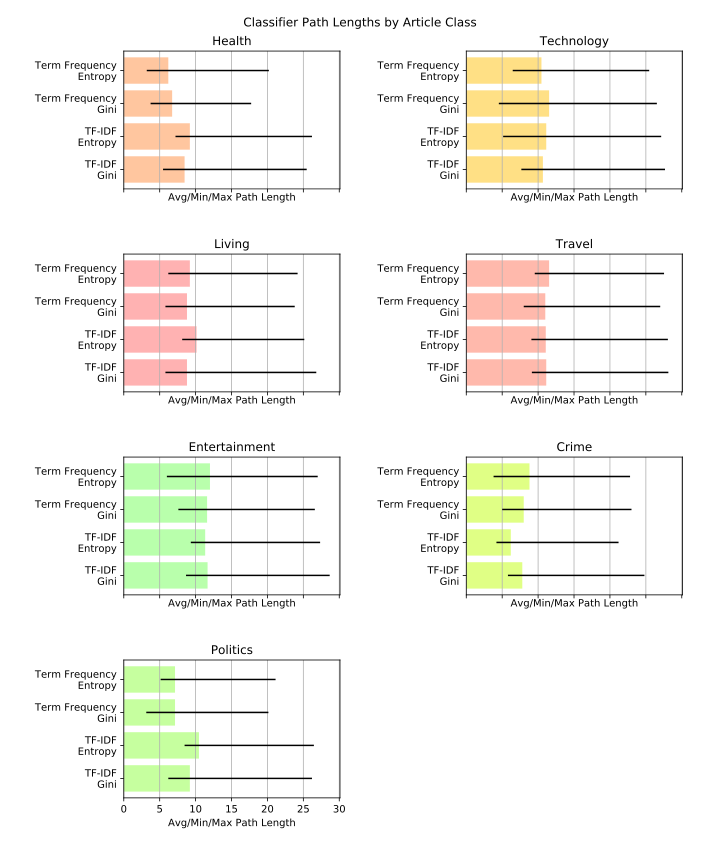
\includegraphics[width=\textwidth]{figures/decision_tree/path_depths}
  \caption{For each article category, the aggregate path lengths over which articles traverse is illustrated.
  Each bar corresponds to the average path lengths in a tree, differentiated by how it was constructed: node splitting criterion (entropy or Gini index) and dataset type (term frequency or tf-idf matrices).
  Error lines correspond to the minimum and maximum path lengths.}
\end{figure}


Figure 1 illustrates the average, minimum, and maximum length of the paths through which an article of a given category traversed to be classified.
From this figure, it is observed that articles from the entertainment, travel, and technology categories required longer paths to perform classifications both on average and at maximum length.
This implies these categories are harder to classify than others.
Beyond those categories, articles from politics, living, and health were the most difficult to classify under entropy-split trees built from the tf-idf representation of the articles.
Crime articles, on the other hand, were the easiest to classify from these trees.
For trees built on term frequency datasets, health and political articles were the easiest to classify.

Figures 2a and 2b illustrate the performance metrics obtained using term frequency and tf-idf representations for training, respectively.
Accuracy, precisions, recalls, and f-scores varied from one criterion-splitting tree to another without a significant overall pattern.

\begin{figure}[h!] \label{fig:perftf_decisiontree}
	\centering
	\begin{subfigure}{.5\textwidth}
	  \centering
	  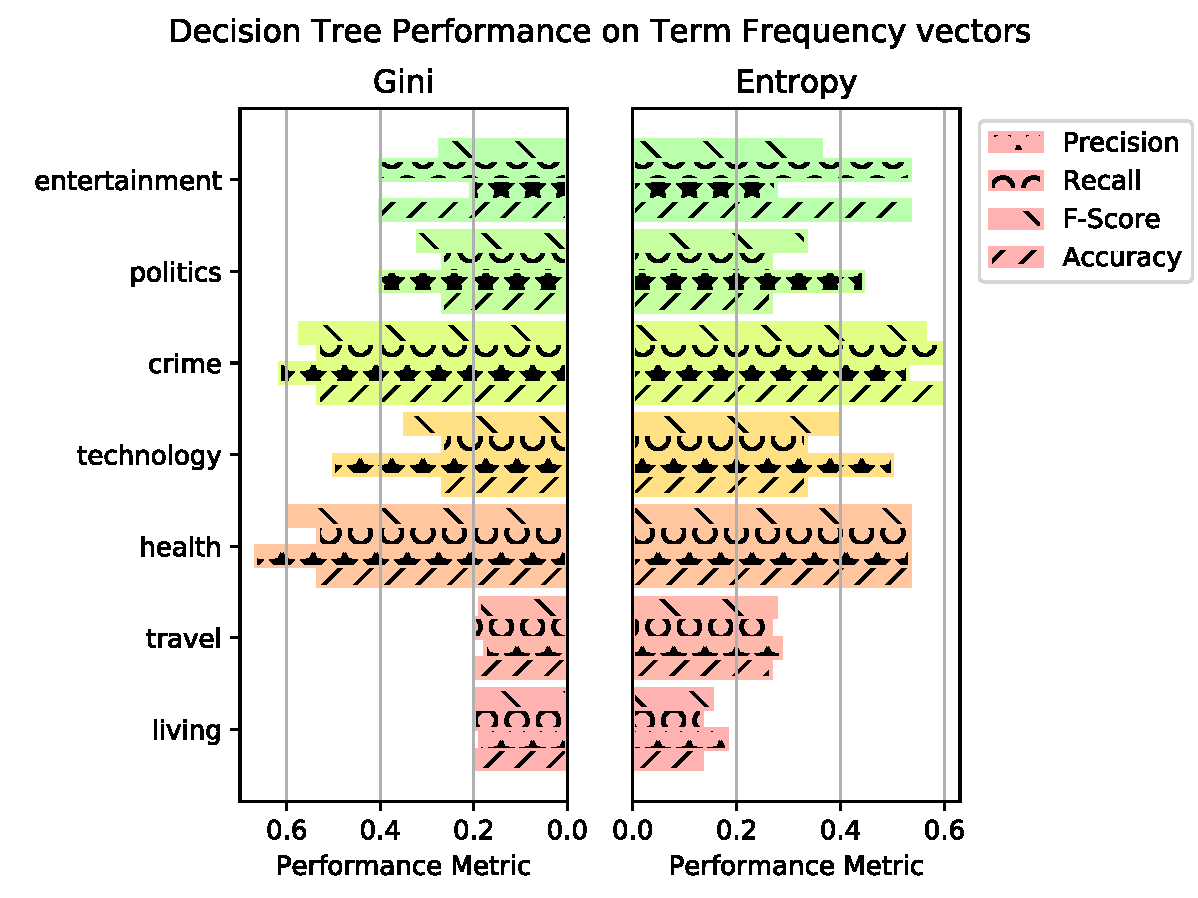
\includegraphics[width=\linewidth]{figures/decision_tree/tf_prec_n_rec}
	  \caption{Performance metrics for Decision Trees trained \\
	  on Term Frequency matrices.}
	  \label{fig:sub1}
	\end{subfigure}%
	\begin{subfigure}{.5\textwidth}
	  \centering
	  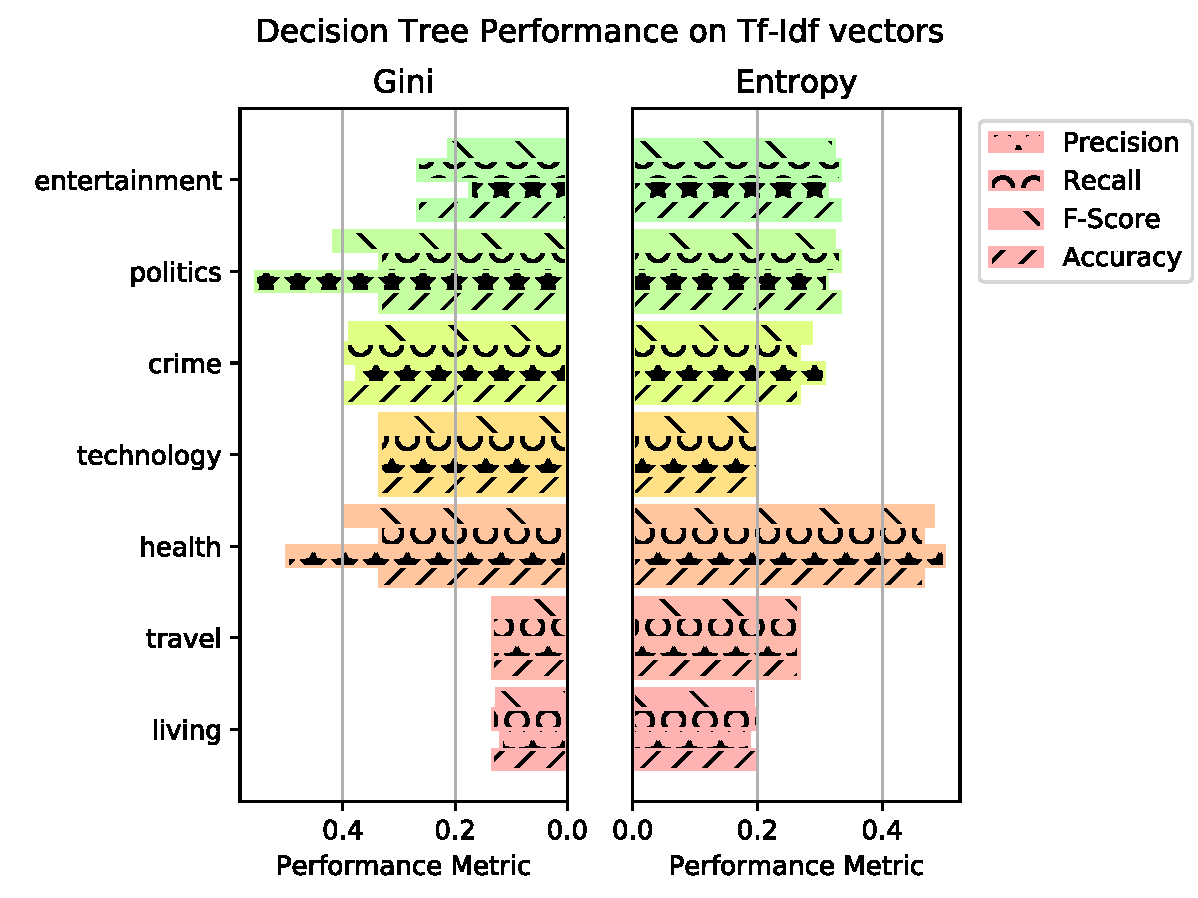
\includegraphics[width=\linewidth]{figures/decision_tree/tfidf_prec_n_rec}
	  \caption{Performance metrics for Decision Trees trained on Tf-idf matrices.}
	  \label{fig:sub2}
	\end{subfigure}
	\caption{Category-specific performance metrics obtained by Decision Tree classification.}
\end{figure}

For decision trees trained on term frequency datasets, accuracies in classification were moderate to low.
Health and crime articles received relatively more accurate classifications than other categories by achieving accuracies above 50\%, with crime articles resulting in the highest accuracy of $\approx$60\% on entropy-split trees.
Travel and living articles, however, were correctly classified at the poorest rate, with performance not exceeding 20\% on any metric (with the exception of travel articles on an entropy-split tree gaining $\approx$30\%).
It should be noted that articles from the living category were successsfully classified by an entropy-splitting tree with approximately the same results as random classification.
Its accuracy, precision, and recall did not exceed 17\%.

Decision trees trained on tf-idf representations of the dataset performed slightly lower than those trained on term frequency representations.
Across all article categories, accuracy and recall did not exceed 50\%.
Politics achieved the highest precision at 58\% under Gini-splitting trees, and health articles obtained an accuracy and recall of $\approx$50\% and a precision of $\approx$57\%.
With the exception of health articles under an entropy-splitting tree, recalls did not exceed 40\%.
Finally, travel and living articles were classified with the worst performance overall, with those on a Gini-splitting tree performing worse than random guessing.


\section{Discussion on k-NN Classification}

The \texttt{KNeighborsClassifier} of the \texttt{scikit-learn} Python library was used to perform the experiments on $k$-Nearest Neighbors ($k$-NN) supervised classification.
This package measures the distance of an article to be classified against the set of articles with known classes, and predicts the article's class based on its $k$-nearest neighbors.
The distance metric and neighbor voting weights are configurable.
For this analyses, voting was uniformly weighted among all $k$ neighbors.
The distance metric was chosen between the Jaccard distance (using the \texttt{jaccard} function defined in the \texttt{scipy.spatial.distance} module), cosine distance (\texttt{cosine} from \texttt{scipy.spatial.distance}), and Euclidean distance (defined in \texttt{scikit-learn} for \texttt{KNeighborsClassifier}).
The vectors to be trained and tested on were either term frequency vectors representing the articles or tf-idf vectors.

\begin{figure}[h!] \label{fig:perf_knn}
	\centering
	\begin{subfigure}{.5\textwidth}
	  \centering
	  \includegraphics[width=\linewidth]{figures/knn/accuracies}
	  \caption{Accuracies obtained by varying the $k$ for $k$-NN\\
	   classification between different vector types and\\
	    different distance metrics.}
	  \label{fig:knn_accuracies}
	\end{subfigure}%
	\begin{subfigure}{.5\textwidth}
	  \centering
	  \includegraphics[width=\linewidth]{figures/knn/fmeasures}
	  \caption{F-measures obtained by varying the $k$ for $k$-NN\\
	   classification between different vector types and different distance metrics, differentiated by the categories to be classified.}
	  \label{fig:knn_fmeasures}
	\end{subfigure}
	\caption{Accuracies and F-measures obtained from the $k$-NN series of experiments.}
\end{figure}

Figures 3a and 3b illustrate the performance changes under varying values of $k$.
The goal of this experiment was to identify the \emph{optimal} $k$ value for performing supervised classifications (Figure 3a), as well as observe the f-measures for each particular article category (Figure 3b).

In the previous report, it was found that the cosine similarity between term frequency vectors performed the best over the Jaccard similarity and Euclidean distance, with Euclidean performing the poorest.
This is corroborated in the bottom plot of Figure 3a.
However, the top plot indicates that transforming a term frequency vector into a tfidf vector brings Euclidean distance almost equal to that of cosine distance.
The Jaccard distance performs the poorest when used between tf-idf vectors, though this is attributed to it not being suitable for real-valued vectors.

By varying the value of $k$, the best performance is achieved at $k=5$ and $7$ for tf-idf vectors, with performance dipping slightly at $8 \le k \le 10$.
For term frequency vectors, the best performance seems to come at $k=4$, with performance dropping from either side.
Intuitively, this suggests that $k<4$ is susceptible to noise and poor correlations between feature occurrences in nearby articles.
For $k>4$, the drop of performance in using the cosine distance indicates that articles are being incorrectly classified by further-away neighbors of different classes.

Looking at Figure 3b, the f-measures for each classification is plotted against the changes to $k$.
Overall, entertainment and living articles receive the worst classifications in both their term frequency and tf-idf representations, implying they have lower precision and recalls, with living articles being the worst of the two.
Crime articles, on the other hand, are consistently classified correctly.
For low $k$ values, the tfidf representation of technology articles achieves better classifications over others, and the term frequency representation of crime articles show similar performance.

For term frequency vectors, when $k$ increases towards 10, articles from entertainment, health, living, and travel begin to suffer, whereas crime remains somewhat consistent.
This seems to indicate that crime articles may form a somewhat exclusive cluster in the term frequency space for its representative features.
For tf-idf vectors, the recorded f-measures remains somewhat stable as $k$ increases, potentially implying that each class of articles might form their own clusters with little diversity in the tf-idf space.

\begin{figure}[h!] \label{fig:heatmap_neighborhoods}
  \centering
  \includegraphics[width=\textwidth]{figures/knn/knn_heatmaps}
  \caption{}
\end{figure}

Figure 4 presents an illustration of the feature occurrences between two articles and the articles within their nearest neighbors.
This figure was created from the experment on 5-nearest neighbors using cosine distance between tf-idf vectors, of which Figure 3 indicates this configuration achieved the very good performance.
For each figure, the first article represents the article to be classified, with the remaining five articles being within each article's $k$-neighborhood.

The top figure shows the article with the most densely populated neighborhood - i.e. the article with $k$ neighbors whose summed distances is minimum across all other articles.
From this figure, we see that it's closest neighbor is within the same class, and shares many common features, the most prominent being the term \emph{drug}.
It is interesting to observe that the remaining neighbors are relatively far away, indicative of their fewer common features and their different categories.
This implies that the tf-idf vector space is relatively sparse.
However, each article still shares some prominent features, such as \emph{women} and \emph{sexual}, which results in them being closer to the considered article than all others.

The bottom figure shows the article with the most sparsely populated neighborhood - i.e. the article with $k$ neighbors whose summed distances is maximum across all other articles.
Although its first neighbor is relatively far away, the features shared between the two are representative for their category, the most prominent being \emph{music}.
The other neighbors appear to only share terms that are somewhat weak in terms of their classification ability as indicated by the differences in category.

As a final comment, it should be observed that both articles would be incorrectly classified using a uniform voting strategy amoung the k neighbors.
However, a correct classification is obtained using a distance-weighted voting strategy.
This might hint towards the benefit of using a distance-weighted voting strategy for sparse-populated neighborhoods, as there might be more noise in a sparse tf-idf vector space than in densely populated ones.

\bibliography{bibliography}{}
\bibliographystyle{plain}
\end{document}
